\section{Introduction}
Welcome to the second part of the course, in which we delve into the intricate world of \textbf{different neural network architectures}. If things seemed complicated before, they will get even more challenging here. \faSadTear[regular]

Convolutional neural networks (CNN) handles \textbf{structured data}, such as images. Various architectures have been developed, from CNNs to Transformers, each attempting different methods to learn effective representations of structured data. In the case of images, these representations capture \textbf{spatially local dependencies} between pixels.

\textit{To understand convolutional neural networks, think of our brain. When we look at an image, the brain processes it in different parts. At first, it recognises simple things like lines and angles. Then, it moves on to more complicated things, until it understands the complete object.}

\textit{The cells in the brain are like small parts that only look at one part of the image. This helps to focus only on the important things. There are two main types of these cells: some look at small and close things, others look at larger things and care less about the exact position.}

\begin{figure}[!htbp]
    \centering
    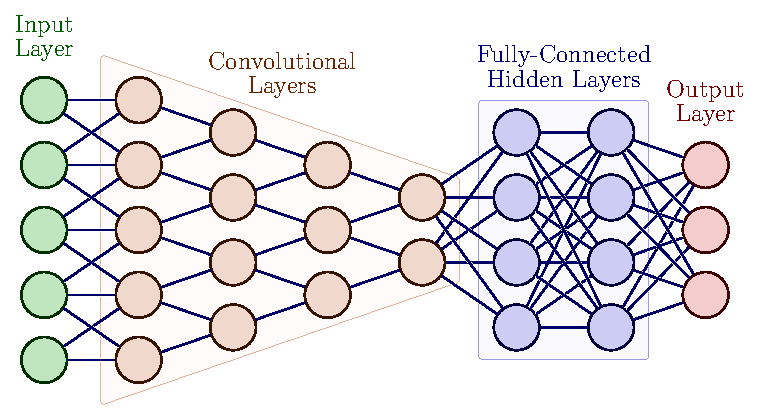
\includegraphics[width=\textwidth]{tikz/chapter5 - CNN.pdf}
    \caption{Example of a Convolutional Neural Network}
\end{figure}

Convolutional neural networks represent a \textbf{specialised version of feedforward neural networks}. If we were to apply a feedforward neural network to process an image, we would lose important information on the spatial relationships between pixels and would have to deal with a large number of parameters due to the need to treat the image as a long input vector. This situation therefore necessitates a complete redesign of the architecture.

CNNs are designed with some specific features, discussed in the previous chapter (section \ref{c4:parameterSharing}), that define their recurrent module. These features include \textbf{local connectivity} and \textbf{weight sharing}, which allow these architectures to effectively capture the spatial characteristics of images without having to manage an excessive number of parameters.

\section{Convolutions}

Convolutional neural networks basically \textbf{replace general matrix multiplication with convolution in at least one of their layers}. A convolutional layer is an operation that takes a matrix (a portion of an image corresponding to the size of the kernel) as input and produces a scalar by calculating the scalar product between the pixel values of the area and the kernel parameters. By progressively moving the kernel, the final output of the convolutional layer will be a matrix. 

Formally, a Convolutional Layer consists of a set of filters, each covering a small spatial portion of the input, known as the \textbf{receptive field}. Each filter is convoluted along the dimensions of the input data, producing a multidimensional feature map representing the filter's responses to various fragments of the input data. \textbf{During training, the network learns filters that are activated in response to specific features at specific spatial locations}.

This concept can be formalised as follows:
$$
S(i,j) = \sum_{m} I(m,n)K(i-m,j-n)
$$
Convolutional layers help to extract local features from an image using filters, which are learnt during training as they store weights. However, in a CNN, filters are not learnt randomly; rather, they are optimised to best fit the architecture, loss function and data.


\begin{figure}[!htbp]
    \centering
    \includegraphics[width=\textwidth]{tikz/chapter5 - Convolution.pdf}
    \caption{Example of a 2D Convolution}
\end{figure}
An example of convolution is shown in the figure above, in which we have this kernel and calculations:

\hspace{0.05\textwidth}
\begin{minipage}{0.4\textwidth}
$$
\begin{pmatrix}
\mathbf{\textcolor{mygreen}{1}} & \mathbf{\textcolor{mygreen}{0}} & \mathbf{\textcolor{mygreen}{1}} \\[-0.2cm]
\mathbf{\textcolor{mygreen}{0}} & \mathbf{\textcolor{mygreen}{1}} & \mathbf{\textcolor{mygreen}{0}} \\[-0.2cm]
\mathbf{\textcolor{mygreen}{1}} & \mathbf{\textcolor{mygreen}{0}} & \mathbf{\textcolor{mygreen}{1}} \\
\end{pmatrix}
$$
\end{minipage}
% \hspace{0.05\textwidth}
\begin{minipage}{0.4\textwidth}
$$
\begin{aligned}
&\mathbf{\textcolor{myred}{1}} \times \mathbf{\textcolor{mygreen}{1}} + \mathbf{\textcolor{myred}{0}} \times \mathbf{\textcolor{mygreen}{0}} + \mathbf{\textcolor{myred}{0}} \times \mathbf{\textcolor{mygreen}{1}}&\\
+ &\mathbf{\textcolor{myred}{1}} \times \mathbf{\textcolor{mygreen}{0}} + \mathbf{\textcolor{myred}{1}} \times \mathbf{\textcolor{mygreen}{1}} + \mathbf{\textcolor{myred}{0}} \times \mathbf{\textcolor{mygreen}{0}}&\\
+ &\mathbf{\textcolor{myred}{1}} \times \mathbf{\textcolor{mygreen}{1}} + \mathbf{\textcolor{myred}{0}} \times \mathbf{\textcolor{mygreen}{0}} + \mathbf{\textcolor{myred}{1}} \times \mathbf{\textcolor{mygreen}{1}}&=\mathbf{\textcolor{mybluee}{4}}\\
\end{aligned}
$$
\end{minipage}
\hspace{0.05\textwidth}

For the input considered, the convolution is calculated through the scalar product between the kernel values and the corresponding input values. 
The result of this calculation is 4, which represents the output of this specific convolution.

It is important to know two fundamental parameters used to control the size of the convolution output and influence the size and shape of the features extracted by the convolutional neural network, namely:
\begin{itemize}
    \item \textbf{Padding}: Padding refers to the addition of values (commonly zeros) around the edges of the input image before applying the convolution. This is useful for controlling the size of the convolution output. Padding may be "\textbf{Valid}" (no padding) or "\textbf{Same}" (padding so that the output is the same size as the input).
    \item \textbf{Stride}: The stride indicates the number of pixels in which the filter (kernel) is moved along the input image during the convolution operation. \textbf{A stride value greater than one} results in a larger displacement, reducing the size of the output. \textbf{A stride value of one} is the most common and produces an output with the same size as the input.
\end{itemize}


The output of the convolutional layer depends on the size of the kernel $K$ and the stride $S$, and can be calculated using the formula $\mathbf{\frac{(N-K)}{S}+1}$, where $N$ is the size of the input. In the case of our example, the input is a square matrix of size 7x7 and the kernel is 3x3, so the output will be a matrix of size 5x5.

However, in some applications, it is convenient to \textbf{keep the size of the output of the convolution equal to the size of the input}. This is achieved through \textbf{zero-padding}: zeros are added around the edges of the matrix.


\textbf{N.B.} It is important to note that when we speaks of "two-dimensional convolutions", we are actually working with three-dimensional tensors. Thus, the example of the two-dimensional convolution given above does not fully reflect the complexity of convolutions in CNNs. In fact, when exploring various architectures, such as AlexNet or VGGNet, it is evident that the drawings of the various layers show the use of three-dimensional tensors. If you want to try and explore this further, here is a useful link that shows what these convolutions actually look like visually: \underline{\href{https://animatedai.github.io/}{Animated AI Convolution}}.


\section{Layers of a CNN}

\begin{remark}{accent}{accent!20}
\textbf{Input image}: This layer represents the raw image entering the network. Generally, images are represented as multidimensional arrays of pixels, where each pixel has a value indicating its light intensity or colour.
\end{remark}

\begin{remark}{mybluee}{mybluee!20}
\textbf{Convolution layer}: This is where the convolution operation takes place, which is fundamental for extracting features from the input image. Here, filters (or kernels) are applied to the image to detect specific patterns. Each filter, as it flows over the entire image, produces a feature map, highlighting the presence of edges, shapes and textures. \textit{It is as if each small region of the image participates in a "discussion" process to identify its unique features, and the different filters carry on this discussion, each highlighting different aspects.} The size of a filter is not constrained, allowing the network to adapt and learn different aspects of the images.
\end{remark}


\begin{remark}{myred}{myred!20}
\textbf{Non-linearity}: After convolution, a non-linear activation function such as ReLU is applied. This layer adds non-linearity to the model, allowing the network to learn and represent complex relationships between image features, without affecting the
receptive fields. 
\end{remark}

\begin{remark}{mygreen}{mygreen!20}
\textbf{Spatial Pooling}: This layer reduces the size of feature maps obtained by convolution, reducing the number of parameters and controlling overfitting. Commonly used are max pooling or average pooling layers, which reduce the size of the feature map by preserving only the most significant values. This also helps to create a spatially invariant representation, as relevant features are preserved even if slightly shifted in the image.
\end{remark}

\begin{remark}{accent!40}{accent!7}
\textbf{Normalisation Layer}: This layer is optional and can be used to normalise feature maps before passing them on to the next layer of the network. As we have seen, normalisation can be useful to ensure that data remain in an appropriate range and to facilitate the network learning process.
\end{remark}

\begin{remark}{accent}{accent!20}
\textbf{Feature Maps}: The feature maps resulting from the previous steps represent the information extracted from the input image. Each feature map corresponds to a specific feature detected by the network and can be interpreted as a simplified representation of the image in terms of relevant patterns and structures. These feature maps are then used as input to subsequent layers of the network for further processing and analysis.
\end{remark}

\section{CNN Architectures (for Classification)}

Let's now discover the main architectures of convolutional neural networks, from the pioneer LeNet to the modern ConvNeXt, which have revolutionised image recognition!

\subsection{LeNet (1998)}
LeNet was the \textbf{milestone that initiated the field of Convolutional Neural Networks}, developed by \textit{Yann LeCun et al.} at AT\&T Labs. Its impact has been instrumental in promoting the use of convolutional neural networks in character recognition and other computer vision applications. Its main features include:
\begin{itemize}
    \item Uses \textbf{convolutional and subsampling} followed by fully connected layers.
    \item \textbf{Requires complete retraining when image resolution changes}.
    \item Paper: \href{http://vision.stanford.edu/cs598_spring07/papers/Lecun98.pdf}{"Gradient-Based Learning Applied to Document Recognition" (LeCun et al.)}
\end{itemize}

\begin{figure}[!htbp]
    \centering
    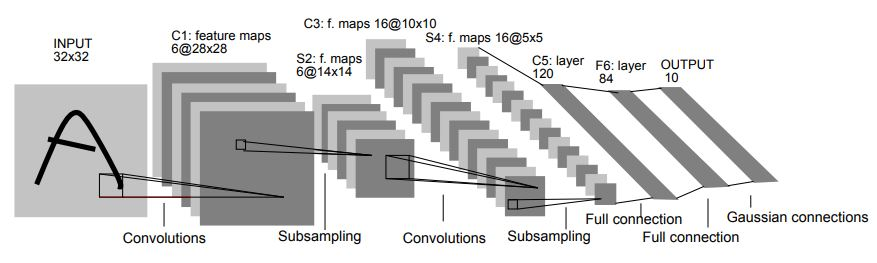
\includegraphics[width=\textwidth]{tikz/chapter5 - LeNet.jpeg}
    \caption{{\color{red}\colorbox{pink}{Tikz TO-DO}} LeNet Architecture}
\end{figure}

\subsection{AlexNet (2012)}
AlexNet marked the \textbf{beginning of the deep learning revolution} and was the first modern CNN architecture. Its main features include:

\begin{itemize}
    \item It has a similar structure to LeNet, but with a \textbf{larger model} (60M parameters) and \textbf{more data}.
    \item It was developed to participate in the \textbf{ImageNet Challenge competition} and demonstrated the effectiveness of CNNs on large datasets.
    \item It was the \textbf{first GPU implementation} of a neural network.
    \item \textbf{Universal Feature Extractor}: AlexNet showed that features learnt from convolutional layers can be generalised and reused effectively for a wide range of computer vision tasks, making it a universal feature extractor.
    \item Paper: \href{https://papers.nips.cc/paper/4824-imagenet-classification-with-deep-convolutional-neural-networks.pdf}{"ImageNet Classification with Deep Convolutional Neural Networks" (Krizhevsky et al.)}
\end{itemize}

\begin{figure}[!htbp]
    \centering
    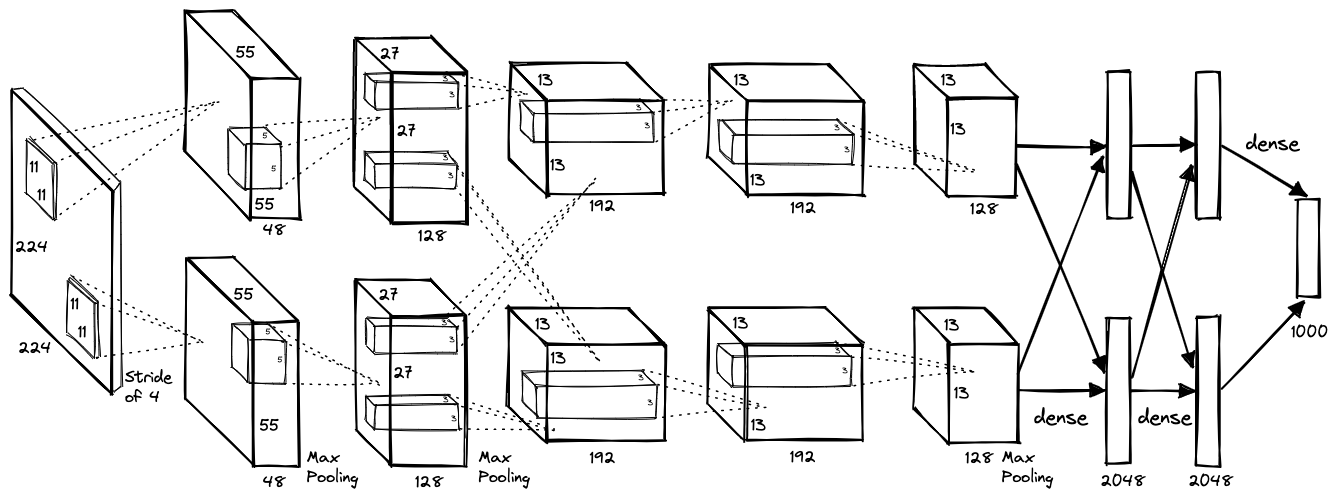
\includegraphics[width=0.9\textwidth]{tikz/chapter5 - AlexNet.png}
    \caption{{\color{red}\colorbox{pink}{Tikz TO-DO}} AlexNet Architecture}
\end{figure}


\subsection{ILSVRC - Zeiler and Fergus Net (2013)}
ILSVRC 2013 introduced similar architecture to AlexNet, but with some significant innovations. Its main features include:
\begin{itemize}
    \item Use of \textbf{large kernels in the first convolutional layers}.
    \item Introduction of the \textbf{explicability of CNNs through deconvolutional networks}.
    \item Use of techniques such as \textbf{Deconvolutional Network} to explain the operation of CNN filters.
    \item Paper: \href{https://arxiv.org/pdf/1311.2901.pdf}{"Visualising and Understanding Convolutional Networks" (Zeiler and Fergus)}
\end{itemize}

\begin{figure}[!htbp]
    \centering
    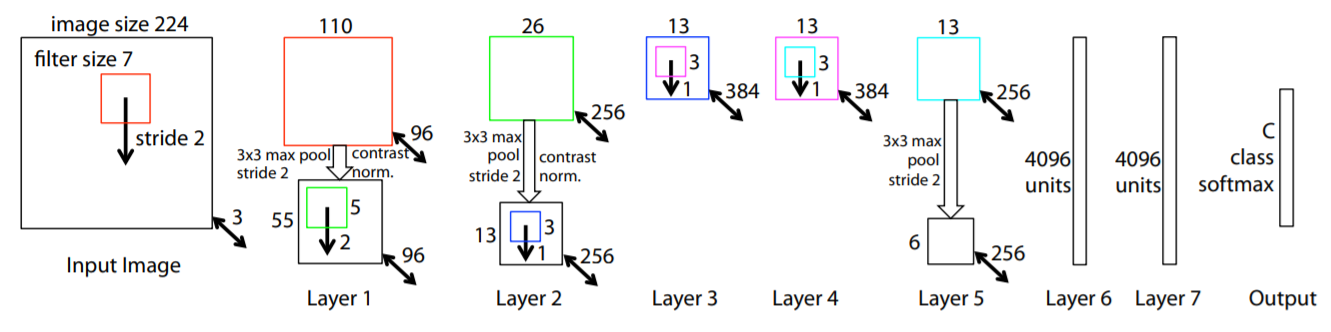
\includegraphics[width=0.9\textwidth]{tikz/chapter5 - ILSVRC.png}
    \caption{{\color{red}\colorbox{pink}{Tikz TO-DO}} ILSVRC Architecture}
\end{figure}

An important technique introduced later to better understand how CNNs work is \textbf{Grad-CAM} (Gradient-weighted Class Activation Mapping), which \textbf{highlights regions of an image that are relevant} for classification.


\subsection{VGGNet (2014)}
VGGNet represents an extension of the ideas introduced by AlexNet, with increased depth. Its main features include:
\begin{itemize}
    \item Very deep architecture with \textbf{more than twice the parameters of AlexNet}.
    \item Keeps the sequence of convolutions, subsamples and layers fully connected.
    \item One of the first architectures to demonstrate that \textbf{network depth is a critical factor for performance}.
    \item Paper: \href{https://arxiv.org/pdf/1409.1556.pdf}{"Very Deep Convolutional Networks for Large-Scale Image Recognition" (Simonyan and Zisserman)}
\end{itemize}

\begin{figure}[!htbp]
    \centering
    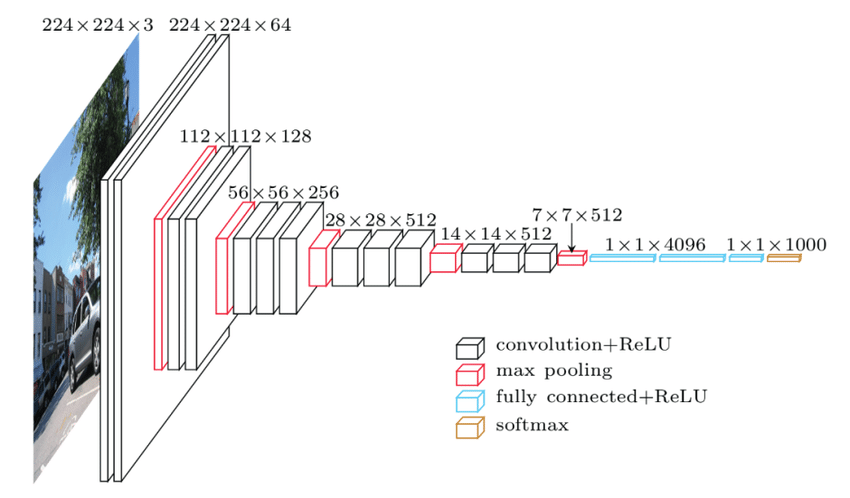
\includegraphics[width=0.7\textwidth]{tikz/chapter5 - VGGNet.png}
    \caption{{\color{red}\colorbox{pink}{Tikz TO-DO}} VGGNet Architecture}
\end{figure}

\subsection{GoogleNet (2014)}
GoogleNet introduced an innovative structure without fully connected layers, reducing the number of parameters compared to AlexNet. Its main features include:
\begin{itemize}
    \item Does not use fully connected layers, \textbf{reducing the complexity of the model} and the risk of overfitting.
    \item Utilisation of \textbf{parallel paths with different receptive field sizes}, allowing the network to capture details at different scales.
    \item Use of \textbf{1x1 convolutions to reduce the number of channels}, improving computational efficiency and reducing the computational workload.
    \item Introduction of \textbf{batch normalisation}, which helps stabilise and speed up the training process.
    \item Paper: \href{https://arxiv.org/pdf/1409.4842.pdf}{"Going Deeper with Convolutions" (Szegedy et al.)}
\end{itemize}

\begin{figure}[!htbp]
    \centering
    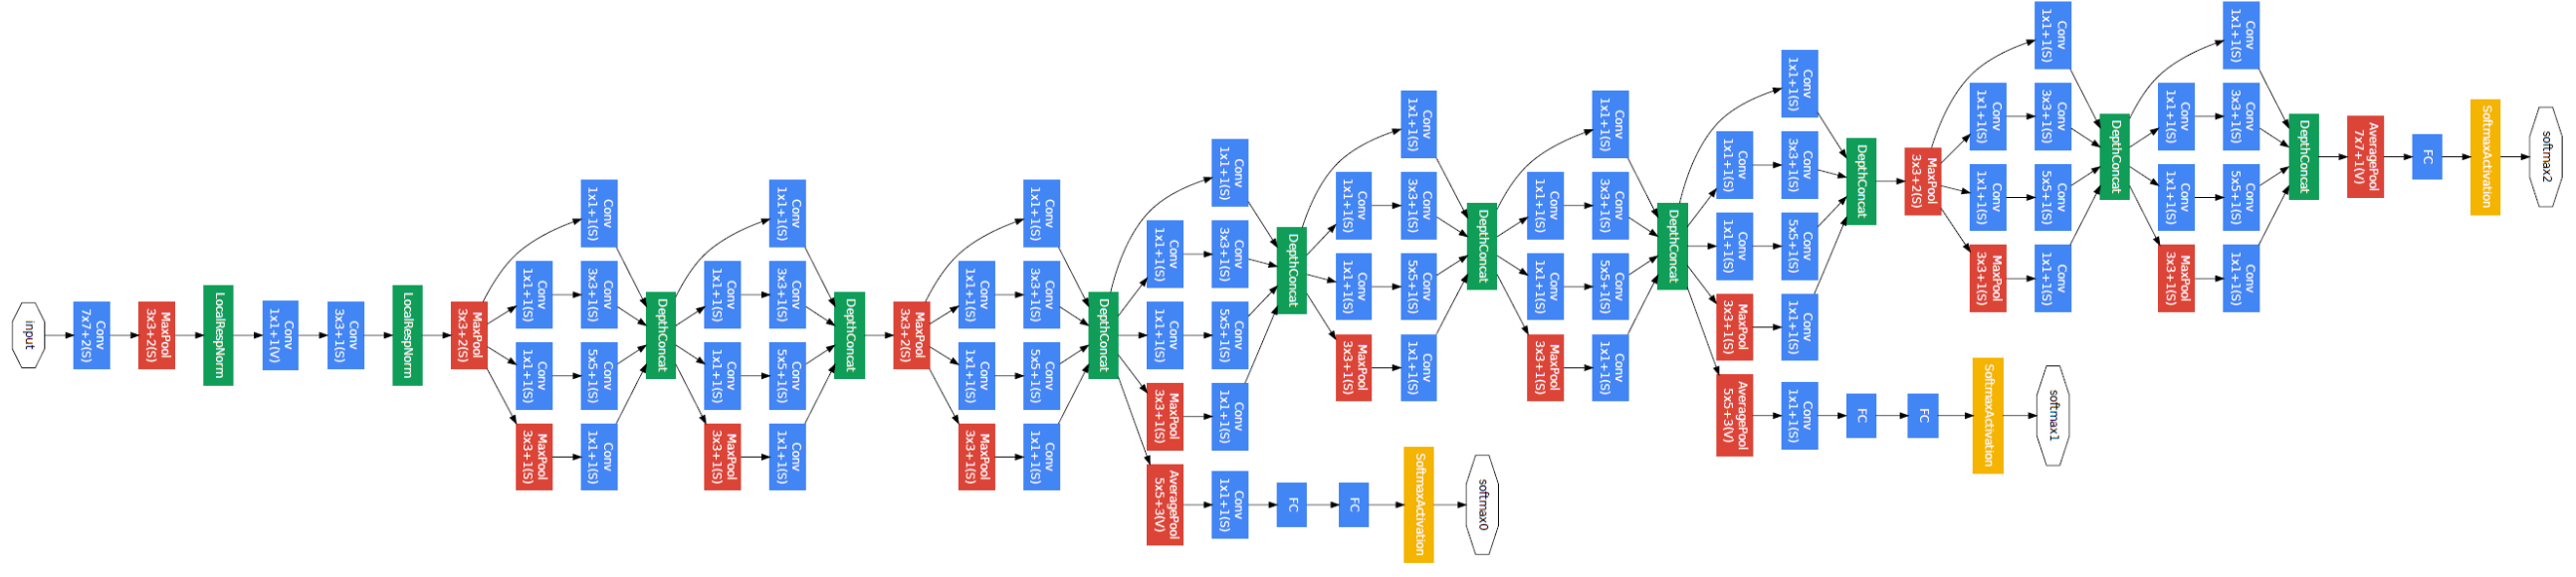
\includegraphics[width=\textwidth]{tikz/chapter5 - GoogleNet.png}
    \caption{{\color{red}\colorbox{pink}{Tikz TO-DO}} GoogleNet Architecture}
\end{figure}


\subsection{ResNet (2015)}
ResNet addressed the problem of \textbf{performance degradation} of deep neural networks by introducing the idea of identity layers, also known as skip connection or identity bypass. Its main features include:
\begin{itemize}
    \item \textbf{Identity Layers}: allow the model to learn to ignore certain layers when they are not needed.
    \item Using \textbf{many small kernels}, reducing the overall number of parameters and improving computational efficiency.
    \item ResNet can be seen as the \textbf{implicit ensemble of more superficial neural networks}, thanks to skip connections.
    \item Skip connections make the \textbf{loss landscape much more uniform} and easier to optimise during the training process.
    \item Paper: \href{https://arxiv.org/pdf/1512.03385.pdf}{"Deep Residual Learning for Image Recognition" (He et al.)}
\end{itemize}

\begin{figure}[!htbp]
    \centering
    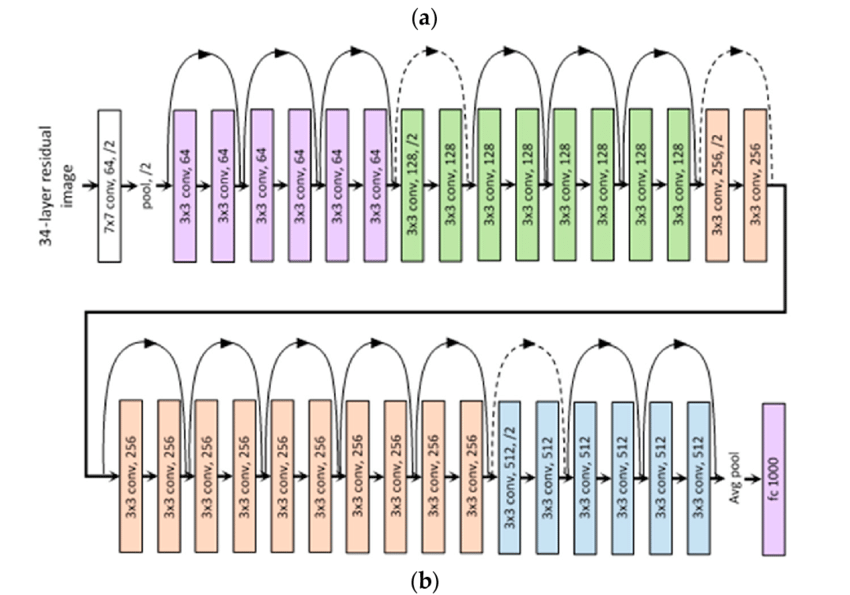
\includegraphics[width=\textwidth]{tikz/chapter5 - ResNet.png}
    \caption{{\color{red}\colorbox{pink}{Tikz TO-DO}} ResNet Architecture}
\end{figure}


There are two remarkable architectures inspired by ResNet: 

\textbf{DenseNet} is an evolution of ResNet that promotes the reuse of features throughout the model, improving gradient propagation and training stability. 

\textbf{SENet} is another evolution of ResNet that recalibrates channel-wise features through Squeeze and Excitation blocks. Squeeze Blocks incorporate global information by calculating the average value of each channel, while Excitation blocks perform adaptive recalibration by calculating a weight for each channel using a sigmoid activation function and multiplying the corresponding channel.


\subsection{ConvNeXt (2022)}
ConvNeXt represents a CNN architecture that has proven to be \textbf{competitive with modern transformers}. Its main features include:
\begin{itemize}
    \item Designed to compete with modern transformer models.
    \item Use of \textbf{connection structures between layers} that enable more effective learning of spatial and semantic relationships.
    \item Paper: \href{https://arxiv.org/pdf/2201.03545.pdf}{"A ConvNet for the 2020s" (Liu et al.)}
\end{itemize}


\section{Regularisation Techniques for CNNs}
Convolutional neural networks have demonstrated excellent learning capability on a wide range of computer vision tasks. However, like many other machine learning techniques, CNNs are \textbf{susceptible to the phenomenon of overfitting}, in which the model overfits the training data, reducing its ability to generalise to new data.

To mitigate overfitting and improve the performance of CNNs, several specific regularisation techniques have been developed. In this section, we will examine some of these popular techniques: Cutout, Dropblock, Cutmix.

\begin{outline}
Cutout is a regularisation technique that consists of \textbf{cutting a random rectangular area of the input image} during the training process. This cut region is subsequently filled with the average pixel value of the entire dataset. \textit{In practice, we force the model to consider more parts of the image during training, thus reducing the risk of overfitting.} \\

Dropblock is an extension of the dropout technique, in which instead of randomly deactivating certain neurons during training, \textbf{entire regions of neurons within a convolutional layer are deactivated}. This prevents the network from focusing too much on specific input features, promoting a more robust and general feature representation. \\

Cutmix: During training, \textbf{a random rectangular area of an image is replaced with a corresponding area from another image}, while class labels are mixed in proportion to the replaced area. This technique encourages the model to learn useful features from multiple regions of the image, while providing a form of regularisation.
\end{outline}


\section{Object Detection}

Image classification is only one of the tasks that convolutional neural networks can tackle. In addition to this, there are more complex tasks such as object detection, in which it is necessary not only to classify the objects in the image, but also to \textbf{identify their exact location through bounding boxes}. In this section, we will explore the strategies used to deal with this challenge using \textit{our beloved} CNNs.

Object detection is a complex task as it requires \textbf{both the classification of objects and the prediction of their positions through bounding boxes}. This makes the training of networks more difficult than simple classification, as there are problems such as data sparsity and difficulty in accurately locating objects.

Before the advent of models such as AlexNet, the situation of object detection was at a standstill, with competition results stable on a plateau. However, the introduction of innovative techniques revolutionised this field.

\subsection{Selective Search for Object Recognition (2013)}
Selective Search is an image segmentation algorithm used to generate \textbf{proposed regions of interest} (RoI) for object recognition. Its main features include:

\begin{itemize}
    \item \textbf{Groups similar pixels together to form regions} and combines them into larger segments.
    \item \textbf{Preliminary Step}: identifies possible areas of the image that might contain objects before proceeding with classification.
    \item Using a hierarchical approach, the algorithm groups pixels according to specific criteria to form a "tree", which is used to obtain bounding boxes.
    \item Paper: \href{https://ivi.fnwi.uva.nl/isis/publications/2013/UijlingsIJCV2013/UijlingsIJCV2013.pdf}{"Selective Search for Object Recognition" (J.R.R. Uijlings et al.)}
\end{itemize}


\subsection{R-CNN - Region-based Convolutional Neural Network (2014)}
R-CNN is the \textbf{first convolutional neural network-based approaches for object recognition}. Its main features include:

\begin{itemize}
    \item \textit{It's nothing but Selective Search + AlexNet}.
    \item Use \textbf{proposed regions} to identify objects in the image.
    \item Uses a convolutional neural network to \textbf{extract features and classify objects within these regions}.
    \item \textbf{Efficiency problem}: R-CNN uses a multi-stage model and Selective Search to explore the entire space of bounding boxes. Also, Selective Search is a "fixed" algorithm that does not dynamically adapt to the image, making it necessary to resize the input before passing it through the neural network, resulting in a \textbf{naive pipeline} approach.
    \item Paper: \href{https://arxiv.org/pdf/1311.2524.pdf}{"Rich feature hierarchies for accurate object detection and semantic segmentation" (Ross Girshick et al.)}
\end{itemize}



\subsection{Fast R-CNN (2015)}
Fast R-CNN is an improved version of R-CNN that \textbf{addresses the efficiency issues} of its predecessor. Its main features include:

\begin{itemize}
    \item \textbf{Region of Interest (RoI) pooling}: Introduces a RoI pooling layer that allows the best use of the information extracted from the convolutional network for each proposed region. This level makes it possible to \textbf{reduce the size of the proposed regions as input} to the final classifier without loss of significant information.
    \item \textbf{Convolution of the forward pass of a CNN}: Fast R-CNN shares the forward pass of a CNN on the image across its selected sub-regions. This means that \textbf{convolution is performed only once} for the entire image, reducing the computational load and improving the overall efficiency of the model.
    \item Paper: \href{https://arxiv.org/pdf/1504.08083.pdf}{"Fast R-CNN" (Ross Girshick)}
\end{itemize}


\begin{figure}[!htbp]
    \centering
    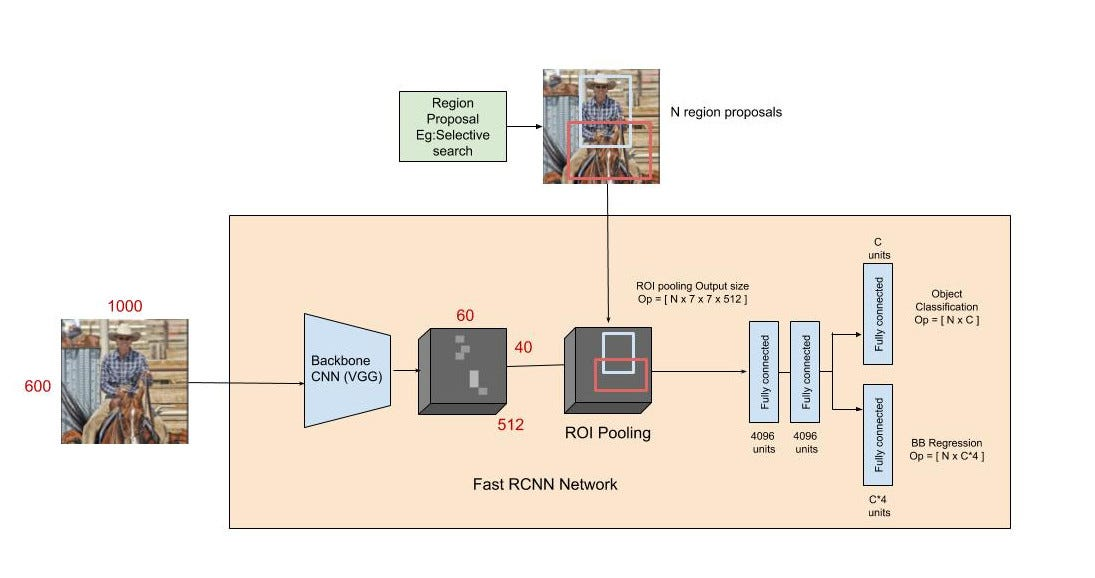
\includegraphics[width=0.8\textwidth]{tikz/chapter5 - Fast R-CNN.jpeg}
    \caption{{\color{red}\colorbox{pink}{Tikz TO-DO}} Fast R-CNN Architecture}
\end{figure}


\subsection{Faster R-CNN (2015)}
Faster R-CNN is another significant development in the field of object detection. Its main features include:

\begin{itemize}
    \item \textbf{Similarity with Fast R-CNN}: Like Fast R-CNN, the image is provided as input to a CNN that provides a convolutional feature map.
    \item \textbf{Use of a separate network for proposal generation}: Instead of using Selective Search, a separate network called RPN (Region Proposal Network) is used in Faster R-CNN to predict region proposals.
    \item \textbf{end-to-end architecture}: With the integration of the RPN module, Faster R-CNN allows the entire end-to-end model to be trained in a single step, improving efficiency and ease of training.
    \item Paper: \href{https://arxiv.org/pdf/1506.01497.pdf}{"Faster R-CNN: Towards Real-Time Object Detection with Region Proposal Networks" (Shaoqing Ren et al.)}
\end{itemize}


\begin{figure}[!htbp]
    \centering
    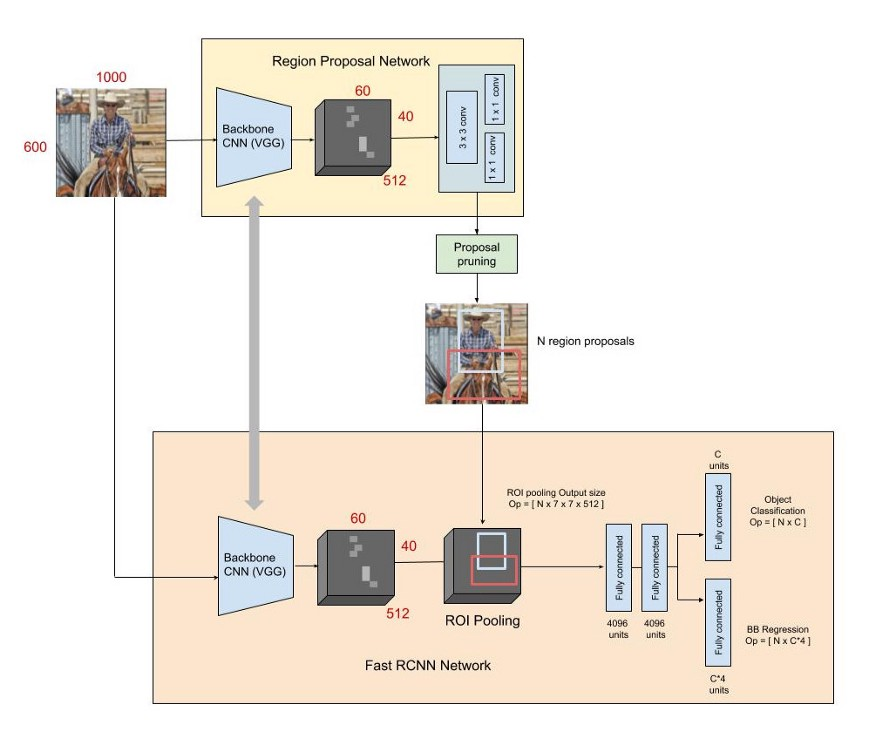
\includegraphics[width=0.65\textwidth]{tikz/chapter5 - Faster R-CNN.jpeg}
    \caption{{\color{red}\colorbox{pink}{Tikz TO-DO}} Faster R-CNN Architecture}
\end{figure}



\subsection{YOLO - You Only Look Once (2016)}
YOLO is an innovative approach to object detection that \textbf{stands out for its speed and efficiency}. Its main features include:

\begin{itemize}
    \item YOLO treats the problem of object detection as a \textbf{direct regression problem}, in which the entire image is divided into a grid and for each grid cell the bounding box and class probability of the objects within that cell are directly predicted.
    \item \textbf{Use of a single convolutional network}: Unlike previous methods that use regions to locate objects in the image, YOLO uses a single convolutional network to predict bounding boxes and class probabilities for these boxes. This makes YOLO's approach simpler and more efficient.
    \item \textbf{Split image into grid}: YOLO splits the image into an SxS grid and for each grid cell predicts a set of bounding boxes. This approach allows YOLO to consider several regions of the image simultaneously.
    \item \textbf{Bounding box selection}: For each predicted bounding box, the YOLO grid produces a class probability and offset values for the bounding box. Bounding boxes with a class probability above a threshold are selected and used to locate the object in the image.
    \item Paper: \href{https://arxiv.org/pdf/1506.02640.pdf}{"You Only Look Once: Unified, Real-Time Object Detection" (Joseph Redmon et al.)}
\end{itemize}

\begin{figure}[!htbp]
    \centering
    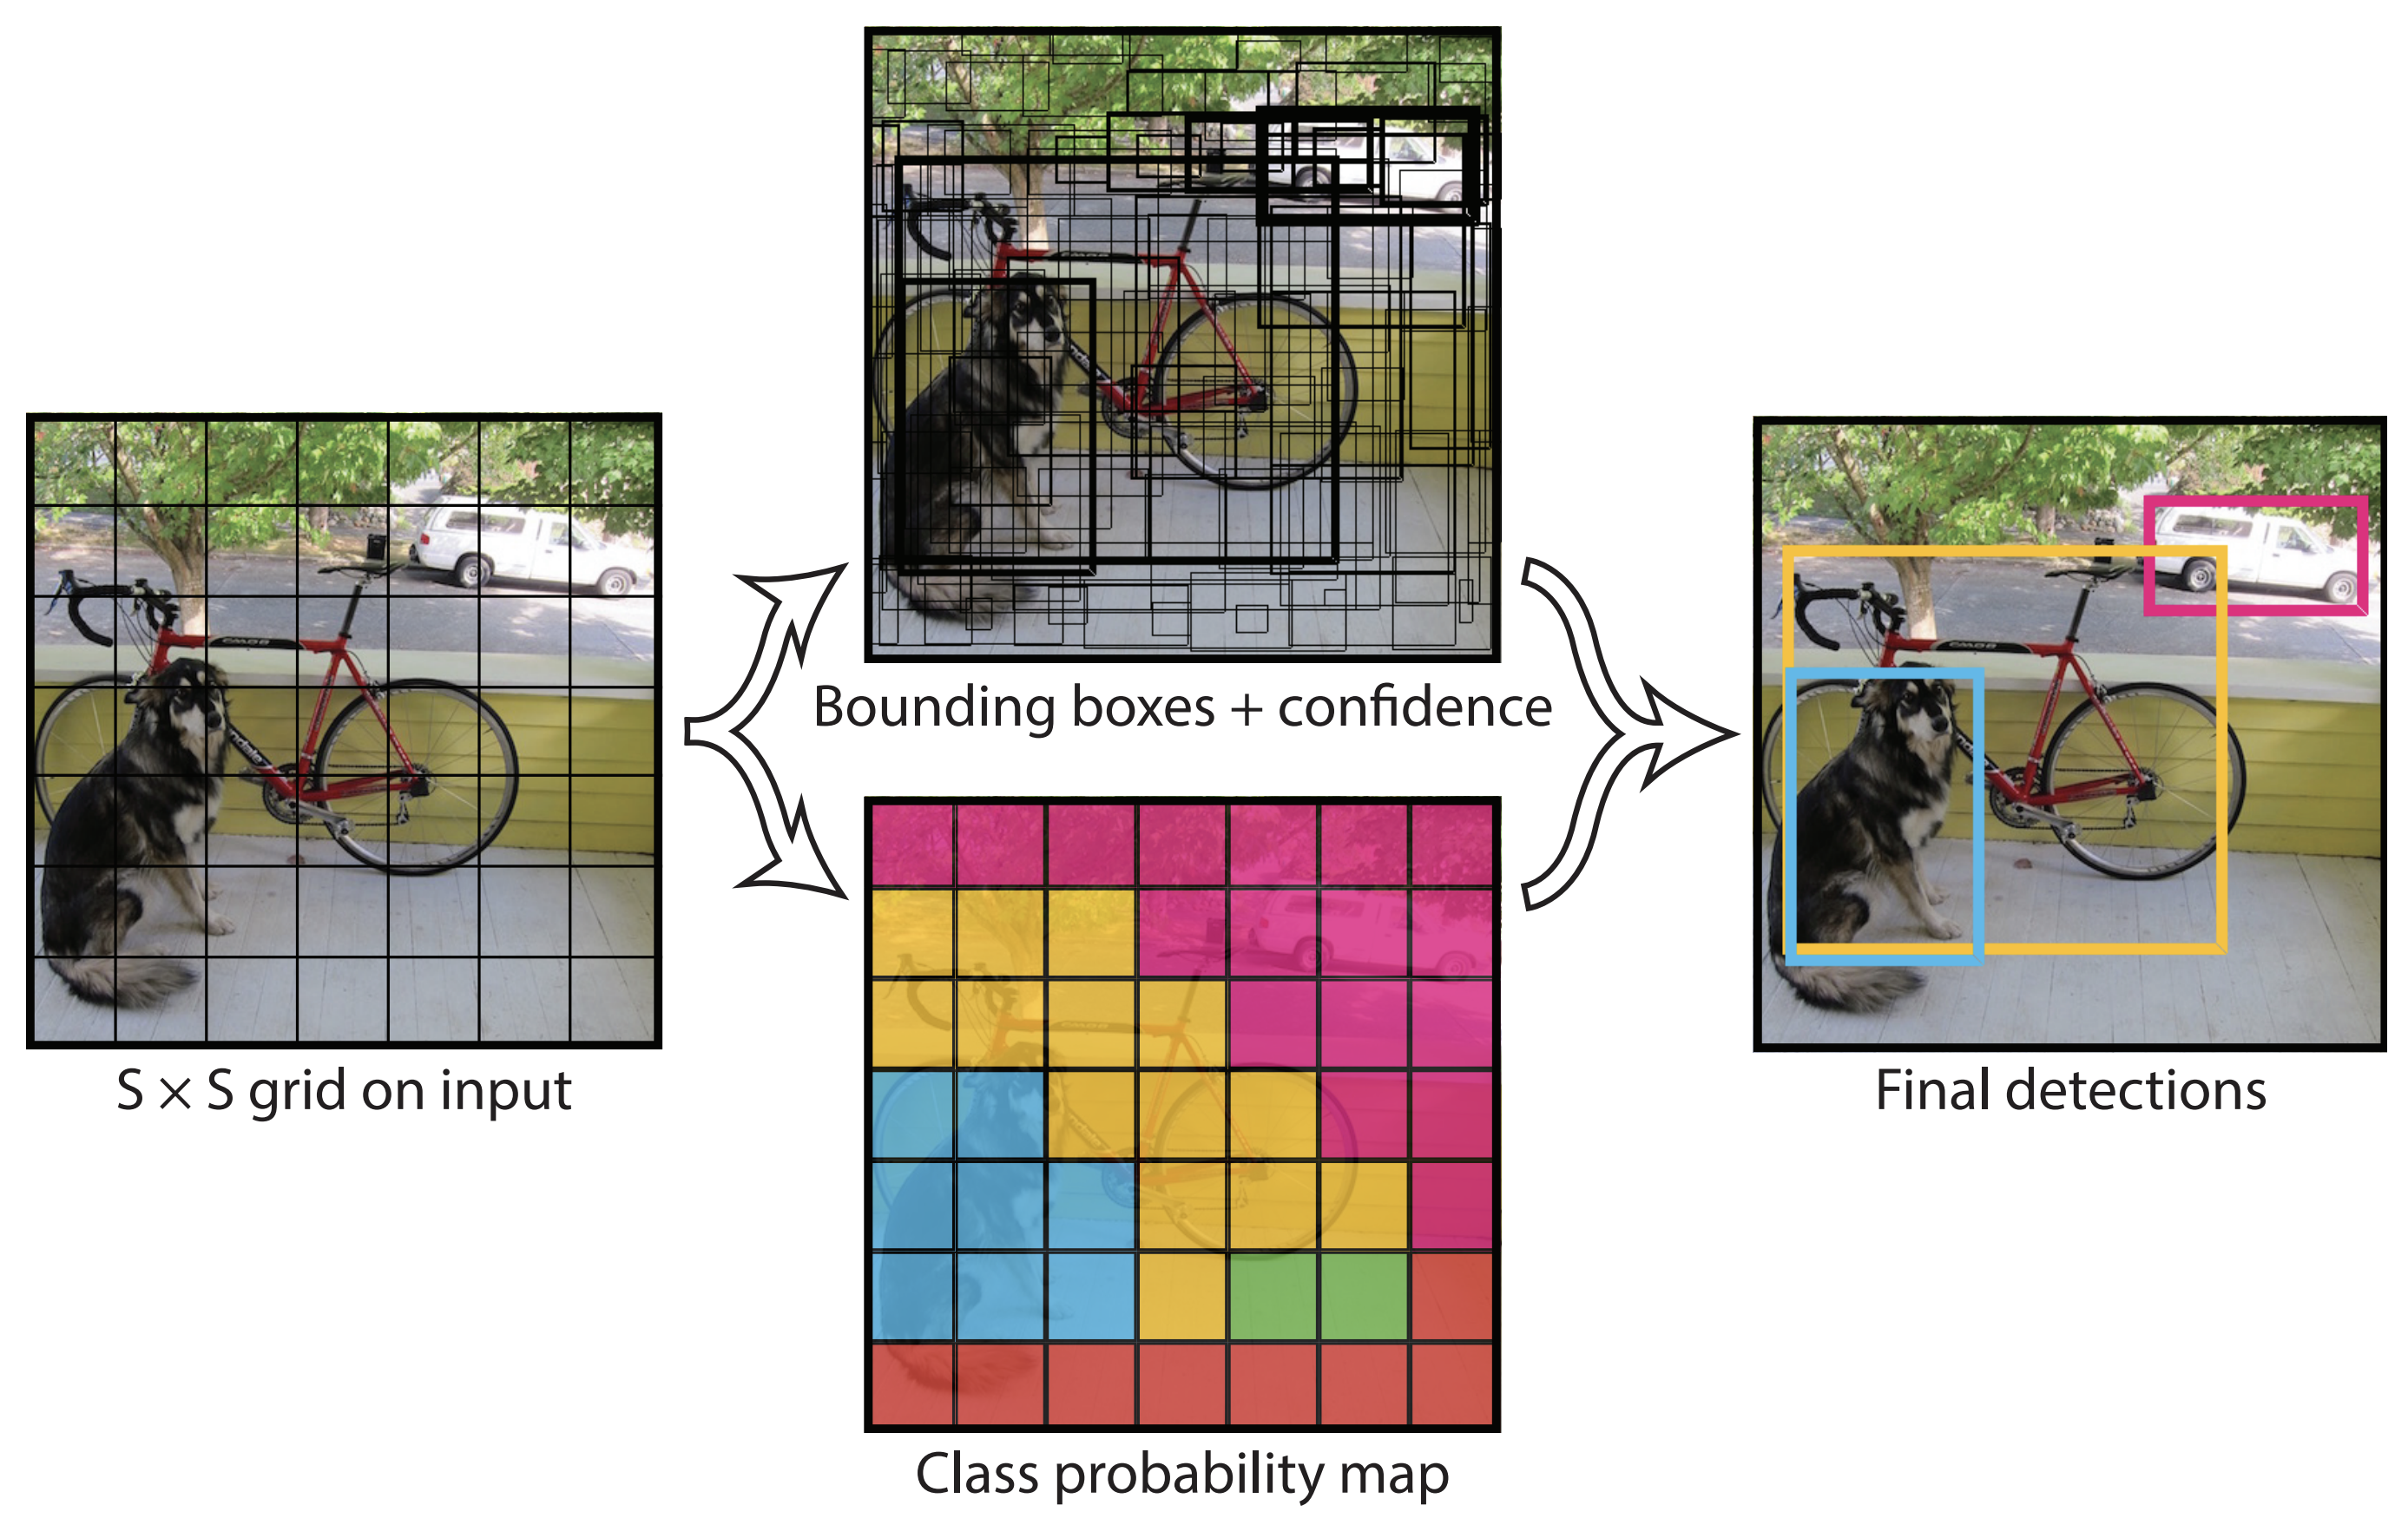
\includegraphics[width=\textwidth]{tikz/chapter5 - YOLO.png}
    \caption{{\color{red}\colorbox{pink}{Tikz TO-DO}} YOLO Architecture}
\end{figure}


\section{Instance Segmentation}

In addition to object classification and bounding box detection, there is another challenge in computer vision: instance segmentation. Instance segmentation consists of \textbf{assigning a label to each pixel of an image}, distinguishing individual objects within the scene. This is an \textbf{even more complex challenge} than simple object detection, as it requires a detailed understanding of the structure and shape of the objects themselves.

One of the most advanced techniques to address this challenge is known as Mask R-CNN, which extends the Faster R-CNN framework for instance segmentation. 

\subsection{Mask R-CNN (2017)}

Mask R-CNN is an extension of Faster R-CNN that adds an \textbf{additional branch to the neural network for instance segmentation}. Its main features include:

\begin{itemize}
    \item Mask R-CNN uses \textbf{RoI Align}, an improved version of RoI Pooling, to ensure more precise alignment of feature maps during the instance segmentation phase. This significantly improves the quality of segmentation masks.
    \item \textbf{Pixel-level segmentation}: Mask R-CNN extends Faster R-CNN for pixel-level segmentation, allowing a label to be assigned to each pixel in the image based on the object instance to which it belongs.
    \item \textbf{FCN added}: Mask R-CNN adds a Fully Convolutional Network on top of selected features to produce accurate and detailed segmentation masks.
    \item Paper: \href{https://arxiv.org/pdf/1703.06870.pdf}{"Mask R-CNN" (Kaiming He et al.)}
\end{itemize}

